\section{Tau Identification with Recurrent Neural Networks}%
\label{sec:tauid_rnn}

The RNN \tauid exploits the discrimination power of both high- and low-level
inputs to distinguish \tauhad from quark- or gluon-initiated jets. This approach
aims to avoid a possible loss of information relevant to \tauid when manually
constructing high-level variables from low-level inputs. Specifically,
charged-particle tracks and topo-clusters in the calorimeters, hereafter
abbreviated as tracks and clusters, are included as low-level inputs to the
algorithm. Their inclusion targets the differences in charged- and
neutral-hadron multiplicities and track- and calorimeter-based isolation between
true and \faketauhadvis. Tau identification is performed separately for 1- and
3-prong \tauhadvis candidates due to their distinct signatures.


\subsection{Input Variables}

The input variables included in the RNN \tauid algorithm are summarised
in~\Cref{tab:tauid_input_variables}. Three categories of inputs are considered:
high-level, track, and cluster inputs. High-level inputs are observables
directly associated to \tauhadvis candidates. Track and cluster inputs refer to
observables of tracks and clusters that are associated to a \tauhadvis
candidate. In the following, a description of the input variable selection and
track/cluster association is given.

\begin{table}[htbp]
  \centering

  \caption[Input variables used for the RNN \tauid.]{Summary of input variables
    used for the RNN \tauid. The local hadronic calibration~\cite{PERF-2014-07}
    is used to calibrate jets, clusters, and \tauhadvis candidates unless
    otherwise noted. Definitions of geometrical topo-cluster moments measuring
    the location and shape of clusters ($\lambda$, $\langle \lambda^2 \rangle$,
    $\langle r^2 \rangle$) are given in Ref.~\cite{PERF-2014-07}. Variables
    using cell-level calorimeter information only consider cells that are part
    of topo-clusters for noise suppression. $\dagger$:~Energy depositions in the
    pre-sampler and first two layers of the electromagnetic calorimeters that
    are part of topo-clusters are abbreviated as ``EM clusters''. The table is
    adapted from Ref.~\cite{ATL-PHYS-PUB-2019-033}.}%
  \label{tab:tauid_input_variables}

  \resizebox{0.99\textwidth}{!}{
    \renewcommand{\arraystretch}{1.3}

\begin{tabular}{clp{13.5cm}}
  \toprule
  & Variable & Description \\
  \midrule
  \parbox[t]{2mm}{\multirow{11}{*}{\rotatebox[origin=c]{90}{High-level inputs\hspace*{65pt}}}}
  & $p_\text{T}$
  & Calorimeter-based estimate of \tauhadvis candidate \pT. \\

  & $f_\text{cent}$
  & Ratio of \ET deposited in calorimeter cells (at EM scale) in cones of $\Delta R < 0.1$ and $\Delta R < 0.2$ about the \tauhadvis axis. \\

  & $f_\text{leadtrack}^{-1}$
  & Ratio of \ET deposited in calorimeter cells (at EM scale) in a cone of $\Delta R < 0.2$ about the \tauhadvis axis and the \pT of the \pT-leading \emph{core} track. \\

  & $\Delta R_\text{max}$
  & Maximum $\Delta R$ between \emph{core} tracks and the \tauhadvis axis. \\

  & $|S_\text{leadtrack}|$
  & Transverse impact parameter significance of the \pT-leading track. Only considered for 1-prong \tauhadvis candidates.\\

  & $S_\text{T}^\text{flight}$
  & Transverse flight path significance. Only considered for 3-prong \tauhadvis candidates. \\

  & $f_\text{iso}^\text{track}$
  & Ratio of the scalar sum of \pT of \emph{isolation} tracks and the scalar sum of \pT of \emph{core} and \emph{isolation} tracks. \\

  & $f_\text{track}^\text{EM}$
  & Ratio of the energy in EM clusters$^\dagger$ and the scalar sum of momenta of \emph{core} tracks. \\

  & $p_\text{T}^\text{EM+track}/\pT$
  & \pT of the \tauhadvis estimated from the momenta of \emph{core} tracks and the two most energetic EM clusters$^\dagger$ divided by the \pT of the calorimetric measurement. \\

  & $m^\text{EM+track}$
  & Invariant mass of the system of \emph{core} tracks and the two most energetic EM clusters$^\dagger$. \\

  & $m^\text{track}$
  & Invariant mass of the system of \emph{core} tracks. Only considered for 3-prong \tauhadvis candidates. \\
  \midrule
  \parbox[t]{2mm}{\multirow{9}{*}{\rotatebox[origin=c]{90}{Track inputs\hspace*{10pt}}}}
  & $p_\text{T}^\text{jet seed}$
  & \pT of the jet seeding the \tauhadvis candidate. \\

  & $p_\text{T}^\text{track}$
  & \pT of the track. \\

  & $\Delta\eta^\text{track}$
  & Difference in $\eta$ between track and \tauhadvis axis. \\

  & $\Delta\phi^\text{track}$
  & Angle between track and \tauhadvis axis in the transverse plane. \\

  & $|d_0^\text{track}|$
  & Absolute value of the transverse track impact parameter. \\

  & $|z_0^\text{track} \sin\theta|$
  & Absolute value of the product of longitudinal track impact parameter and the sine of the polar angle of the track. \\

  & $N_\text{IBL hits}$
  & Number of hits on the track in the IBL. \\

  & $N_\text{Pixel hits}$
  & Number of hits on the track in pixel detector layers. \\

  & $N_\text{SCT hits}$
  & Number of hits on the track in SCT layers. \\

  \midrule
  \parbox[t]{2mm}{\multirow{7}{*}{\rotatebox[origin=c]{90}{Cluster inputs}}}
  & $p_\text{T}^\text{jet seed}$
  & \pT of the jet seeding the \tauhadvis candidate. \\

  & $E_\text{T}^\text{cluster}$
  & \ET of the cluster. \\

  & $\Delta\eta^\text{cluster}$
  & Difference in $\eta$ between cluster and \tauhadvis axis. \\

  & $\Delta\phi^\text{cluster}$
  & Angle between cluster and \tauhadvis axis in the transverse plane. \\

  & $\lambda_\mathrm{cluster}$
  & Longitudinal distance of the cluster barycentre from the calorimeter front face. \\

  & $\langle \lambda^2\rangle_{\text{cluster}}$
  & Second longitudinal cluster moment. \\

  & $\langle r^2\rangle_{\text{cluster}}$
  & Second radial cluster moment. \\
  \bottomrule
\end{tabular}

%%% Local Variables:
%%% mode: latex
%%% TeX-master: "../phd_thesis"
%%% End:

  }
\end{table}

\subsubsection{High-Level Input Variables}

The selection of high-level input variables is based on the variables used in
the BDT-based \tauid algorithm developed by the ATLAS
collaboration~\cite{ATL-PHYS-PUB-2015-045}, which was updated in
Ref.~\cite{cdeutsch-master} for the new \tauhadvis reconstruction techniques
deployed during Run~2 of the LHC. The BDT \tauid uses only the high-level
variables summarised in~\Cref{tab:tauid_input_variables} as inputs and serves as
a baseline for comparison with the RNN-based algorithm.

Variables sensitive to the lifetime and mass of the \taulepton
($|S_{\text{T}}^{\text{flight}}|$, $|S_{\text{leadtrack}}|$,
$m^{\text{track}}$), the isolation of \tauhadvis in the tracking
system ($f_{\text{iso}}^{\text{track}}$) and the calorimeters
($f_{\text{cent}}$), and combinations of track- and calorimeter-based
isolation ($f_{\text{track}}^{\text{EM}}$,
$p_{\text{T}}^{\text{EM+track}} / \pT$) are among the most important
high-level variables included in the \tauid algorithms. Three
exemplary distributions are shown in~\Cref{fig:tauid_high_level_vars}.


\begin{figure}[htbp]
  \centering

  \begin{subfigure}{0.33\textwidth}
    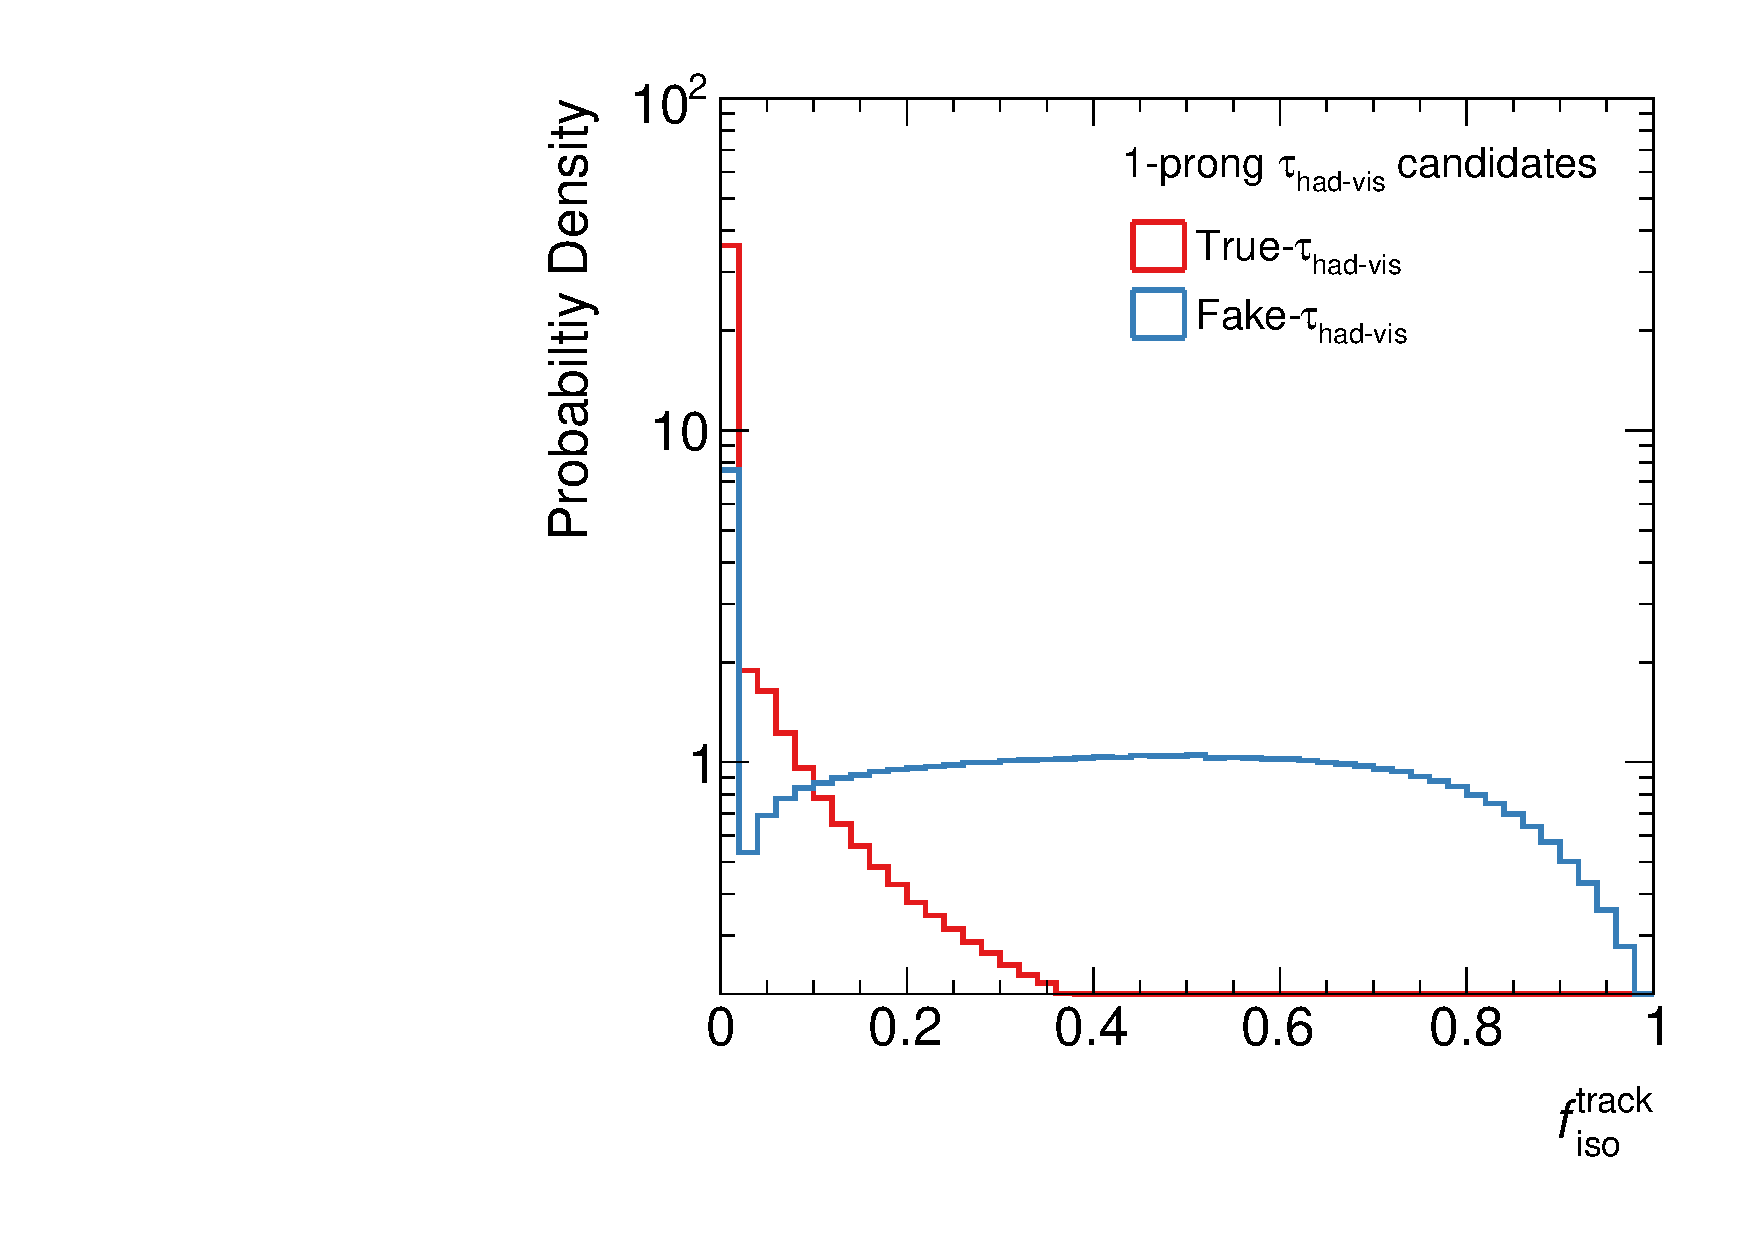
\includegraphics[width=\textwidth]{tauid/invars/invars_sumpttrkfrac_1P}
    \subcaption{}
  \end{subfigure}\hfill%
  \begin{subfigure}{0.33\textwidth}
    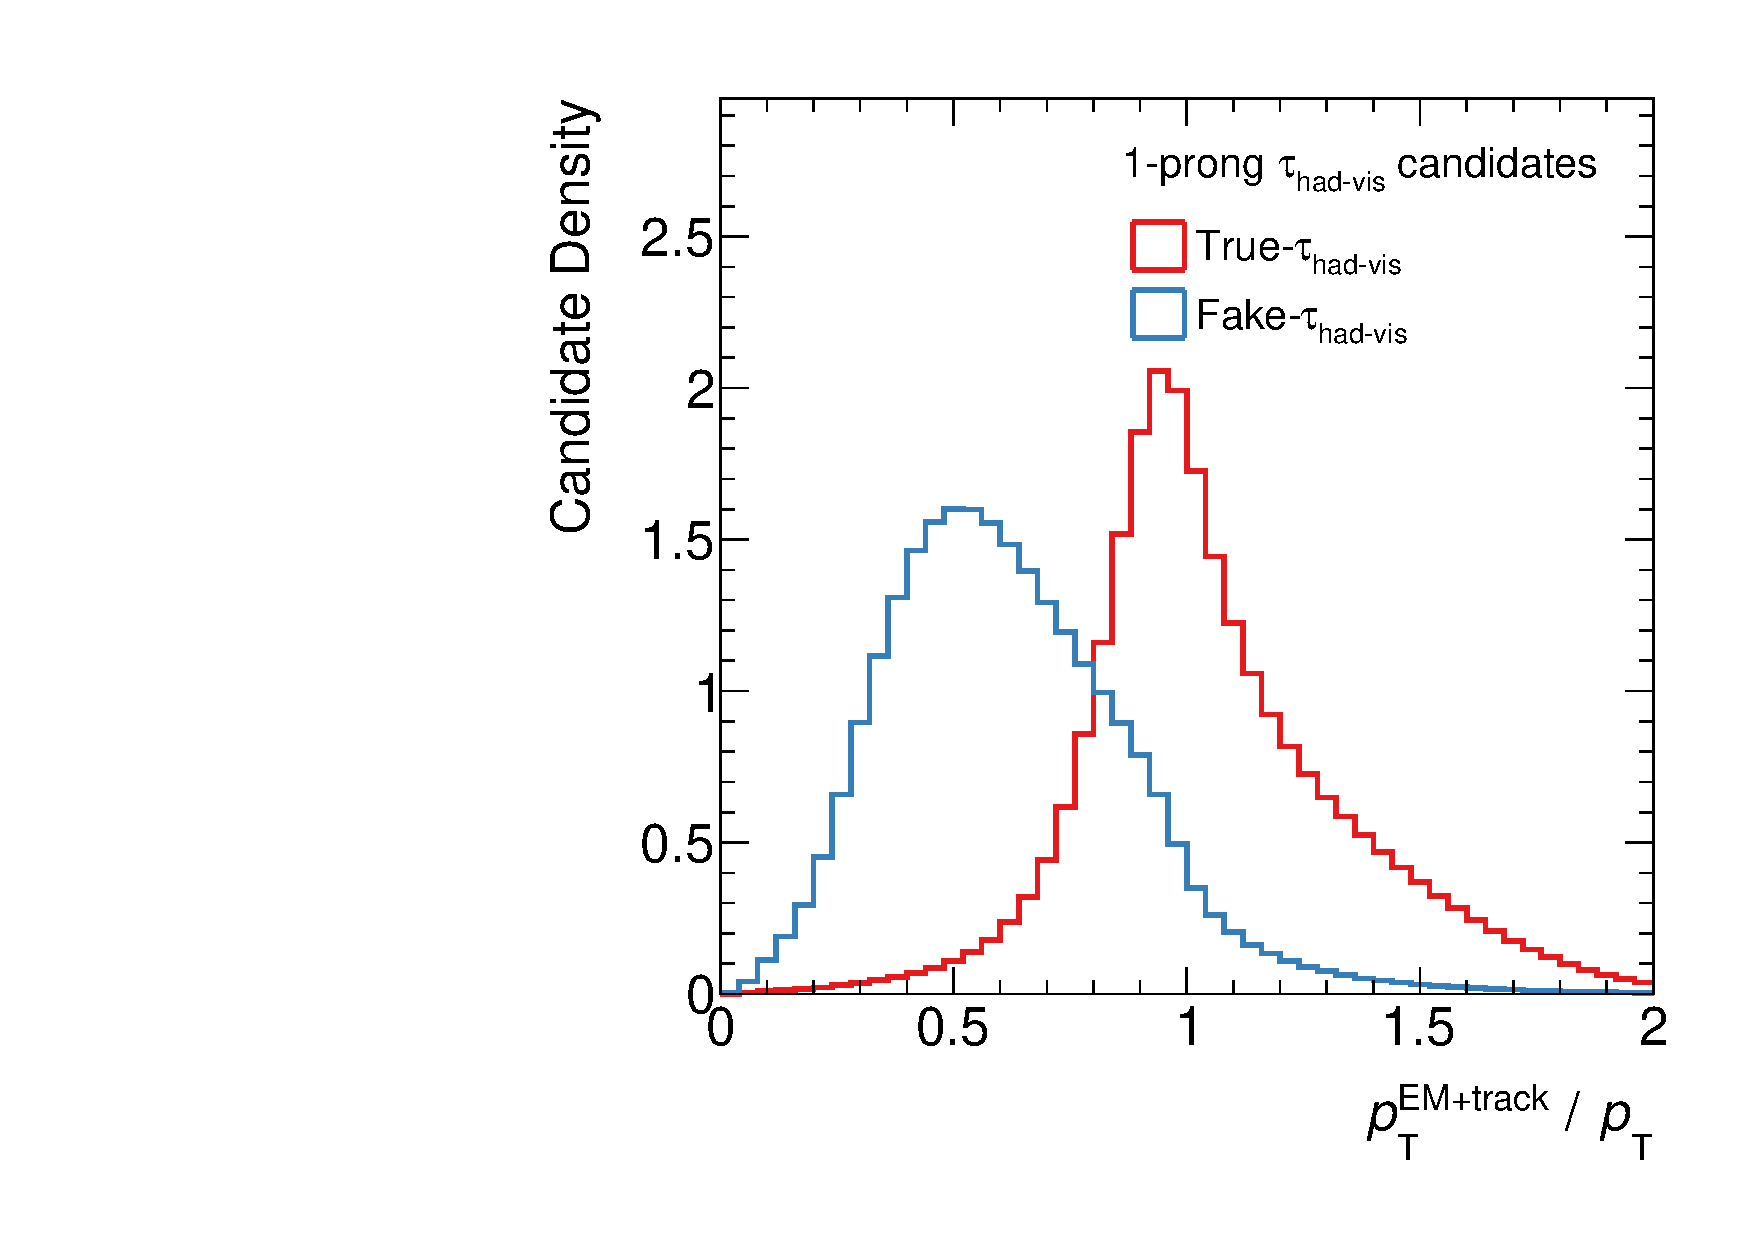
\includegraphics[width=\textwidth]{tauid/invars/invars_ptratioeflowapprox_1P}
    \subcaption{}
  \end{subfigure}\hfill%
  \begin{subfigure}{0.33\textwidth}
    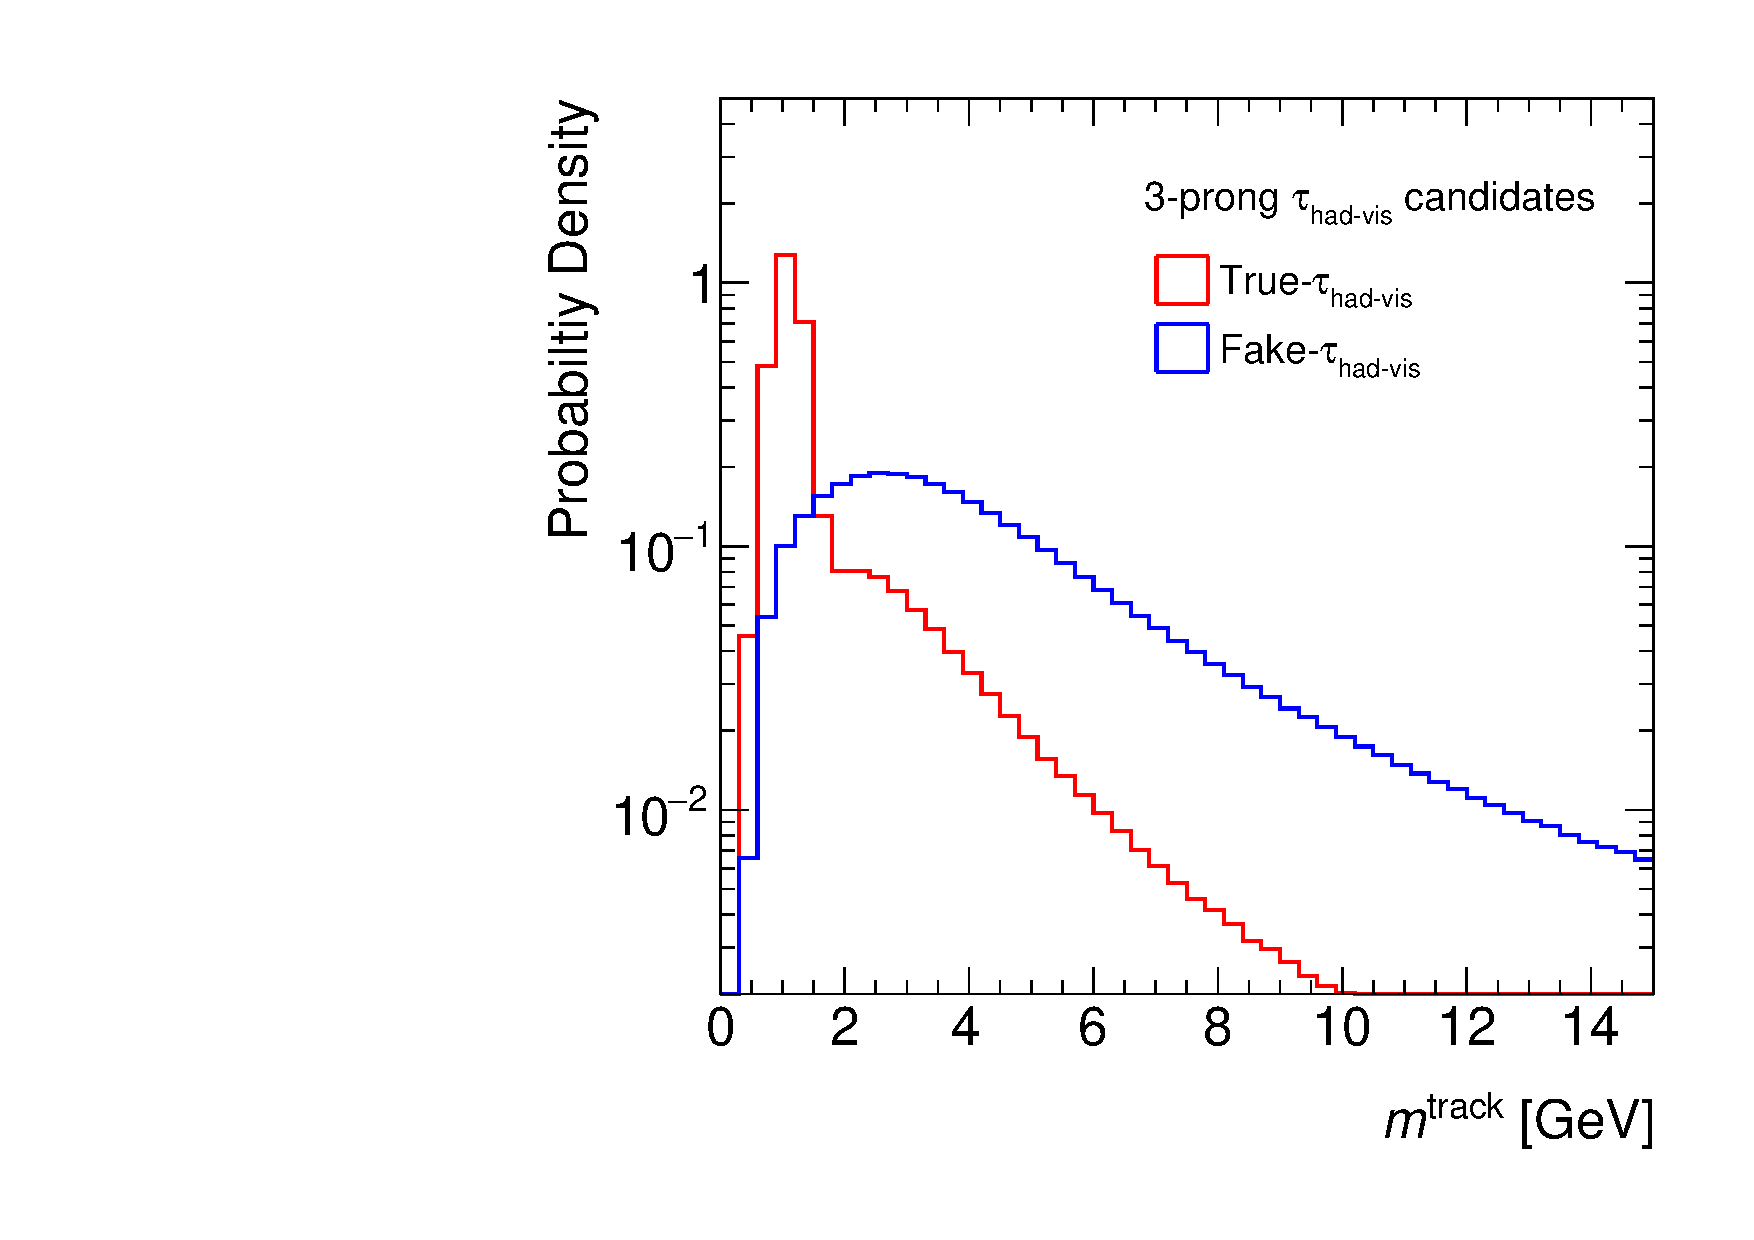
\includegraphics[width=\textwidth]{tauid/invars/invars_masstrksys_3P}
    \subcaption{}
  \end{subfigure}

  \caption[Distributions of exemplary high-level input variables used for
  \tauid.]{Distributions of exemplary high-level input variables used for
    \tauid. (a):~The ratio of the scalar sum of \pT of tracks classified as
    \emph{isolation} with respect to tracks classified as \emph{core} or
    \emph{isolation}. (b):~The ratio of \tauhadvis candidate \pT estimated using
    a simplified particle flow approach and the purely calorimeter-based
    measurement (cf.~\Cref{tab:tauid_input_variables}). (c):~The mass of the
    system of \emph{core} tracks for 3-prong \tauhadvis candidates.}%
  \label{fig:tauid_high_level_vars}
\end{figure}


\subsubsection{Track Input Variables}

Reconstructed tracks with $\pT > \SI{500}{\MeV}$ and within a cone of
$\Delta R < 0.4$ about the \tauhadvis candidate axis are considered as inputs to
the RNN \tauid. No selections are applied on the quality and impact parameters
of reconstructed tracks, thus the inputs include tracks from the \tauleptonC
decay as well as fake tracks and tracks from pile-up. Instead, track quality
criteria ($N_{\text{IBL hits}}$, $N_{\text{Pixel hits}}$, $N_{\text{SCT hits}}$)
and track impact parameters ($|d_0^{\text{track}}|$,
$|z_0^{\text{track}} \sin\theta|$) are included as observables of tracks.

In addition, several other track-level observables, summarised
in~\Cref{tab:tauid_input_variables}, are included. Among the most important
variables are the transverse momenta of reconstructed tracks
($p_{\text{T}}^{\text{track}}$) and their angular separation from the \tauhadvis
candidate axis ($\Delta \eta^{\text{track}}$, $\Delta
\phi^{\text{track}}$). These variables are included to probe the isolation
properties of \tauhadvis candidates. A special case is the
$p_{\text{T}}^{\text{jet seed}}$ variable, the \pT of the jet seeding the
\tauhadvis candidate, which is not a track property but is still included as an
observable for every track. This is done to provide an approximate \pT-scale of
the jet already at the level of individual input tracks. Exemplary distributions
of the transverse momenta of the three highest-\pT tracks normalised to
$p_{\text{T}}^{\text{jet seed}}$ are shown
in~\Cref{fig:tauid_low_level_variables_track} for 1-prong \tauhadvis
candidates.%\todo{Add 2D plots in appendix?}

% \todo[inline]{It would be nice to have 2D plots of leading track \pT vs
% sub-leading track \pT in the appendix. Same for cluster \ET.}

\begin{figure}[htbp]
  \centering

  \begin{subfigure}{0.33\textwidth}
    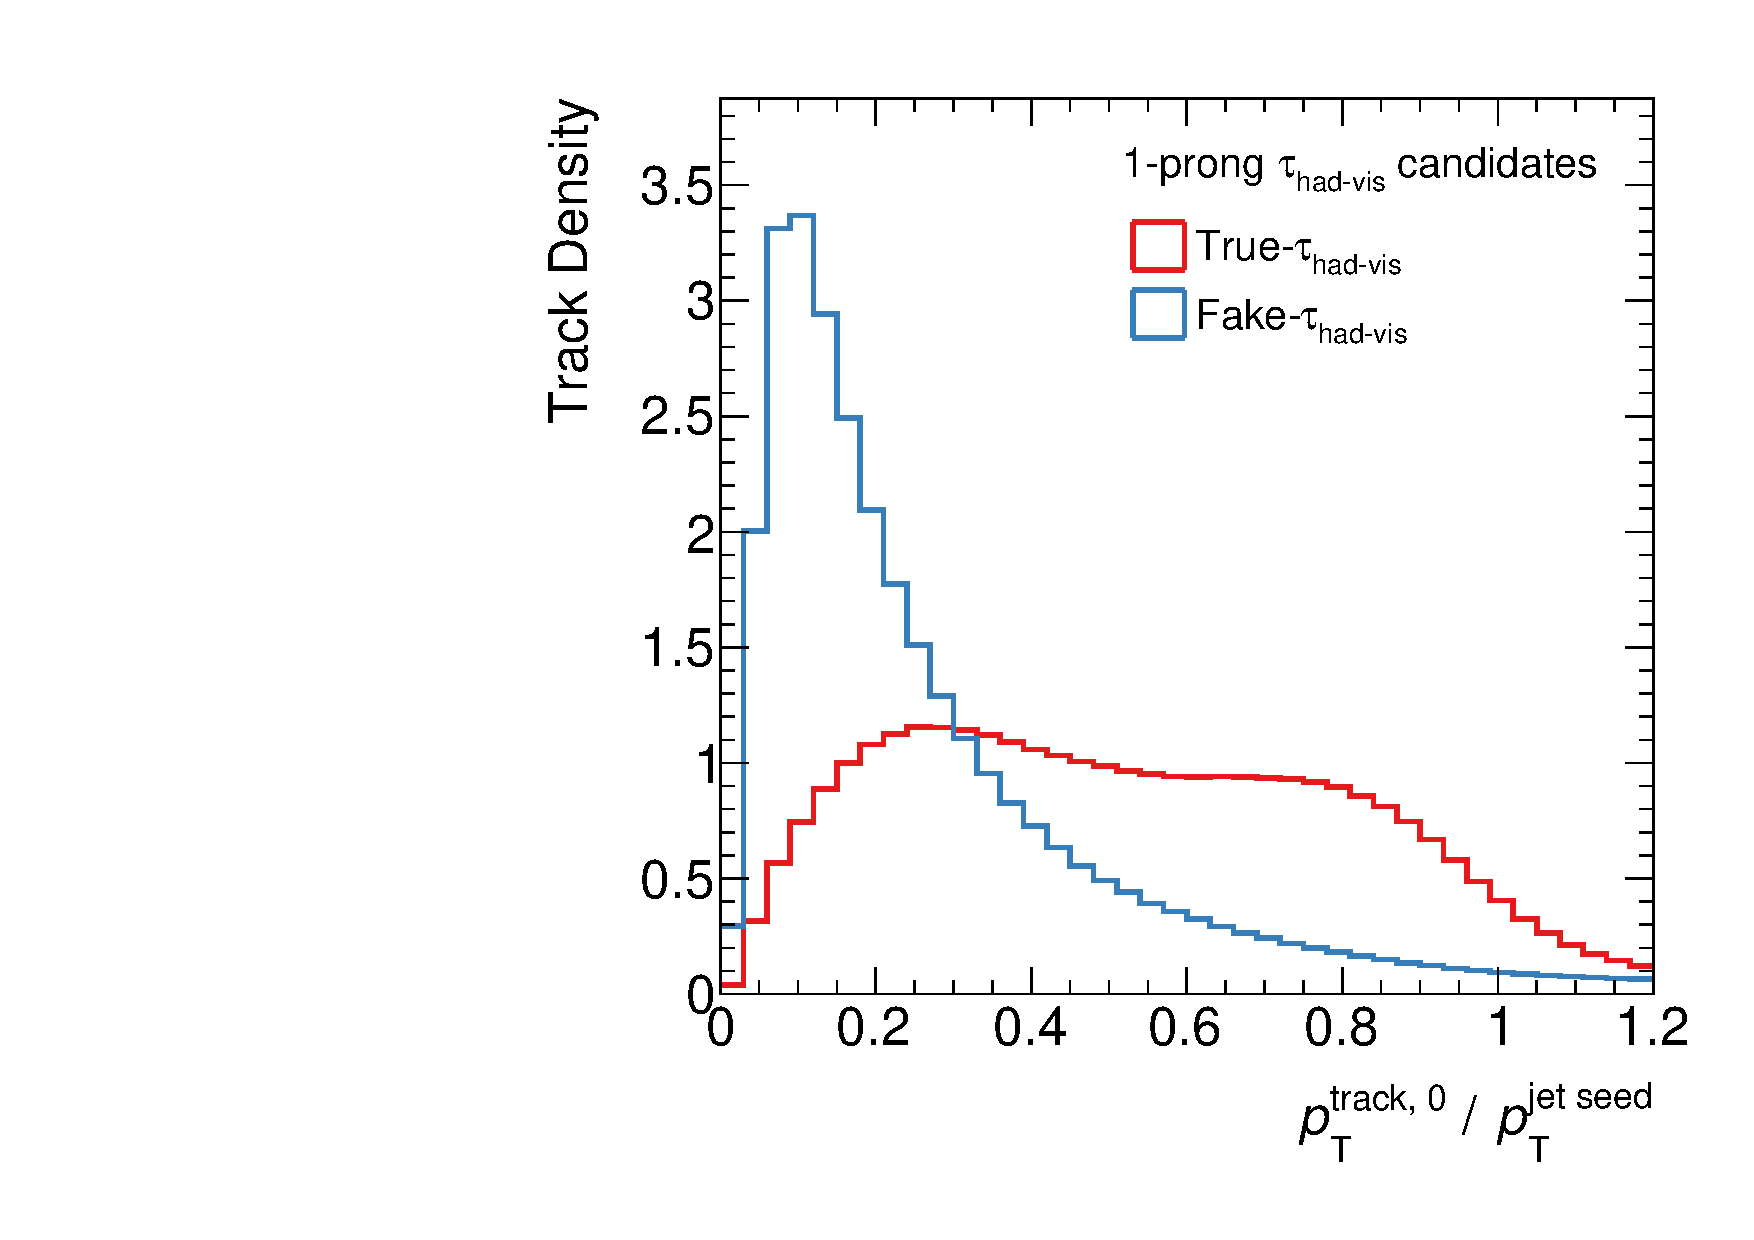
\includegraphics[width=\textwidth]{tauid/invars/invars_trk0relpt_1P}
    \subcaption{}%
    \label{fig:tauid_low_level_variables_track0}
  \end{subfigure}%
  \begin{subfigure}{0.33\textwidth}
    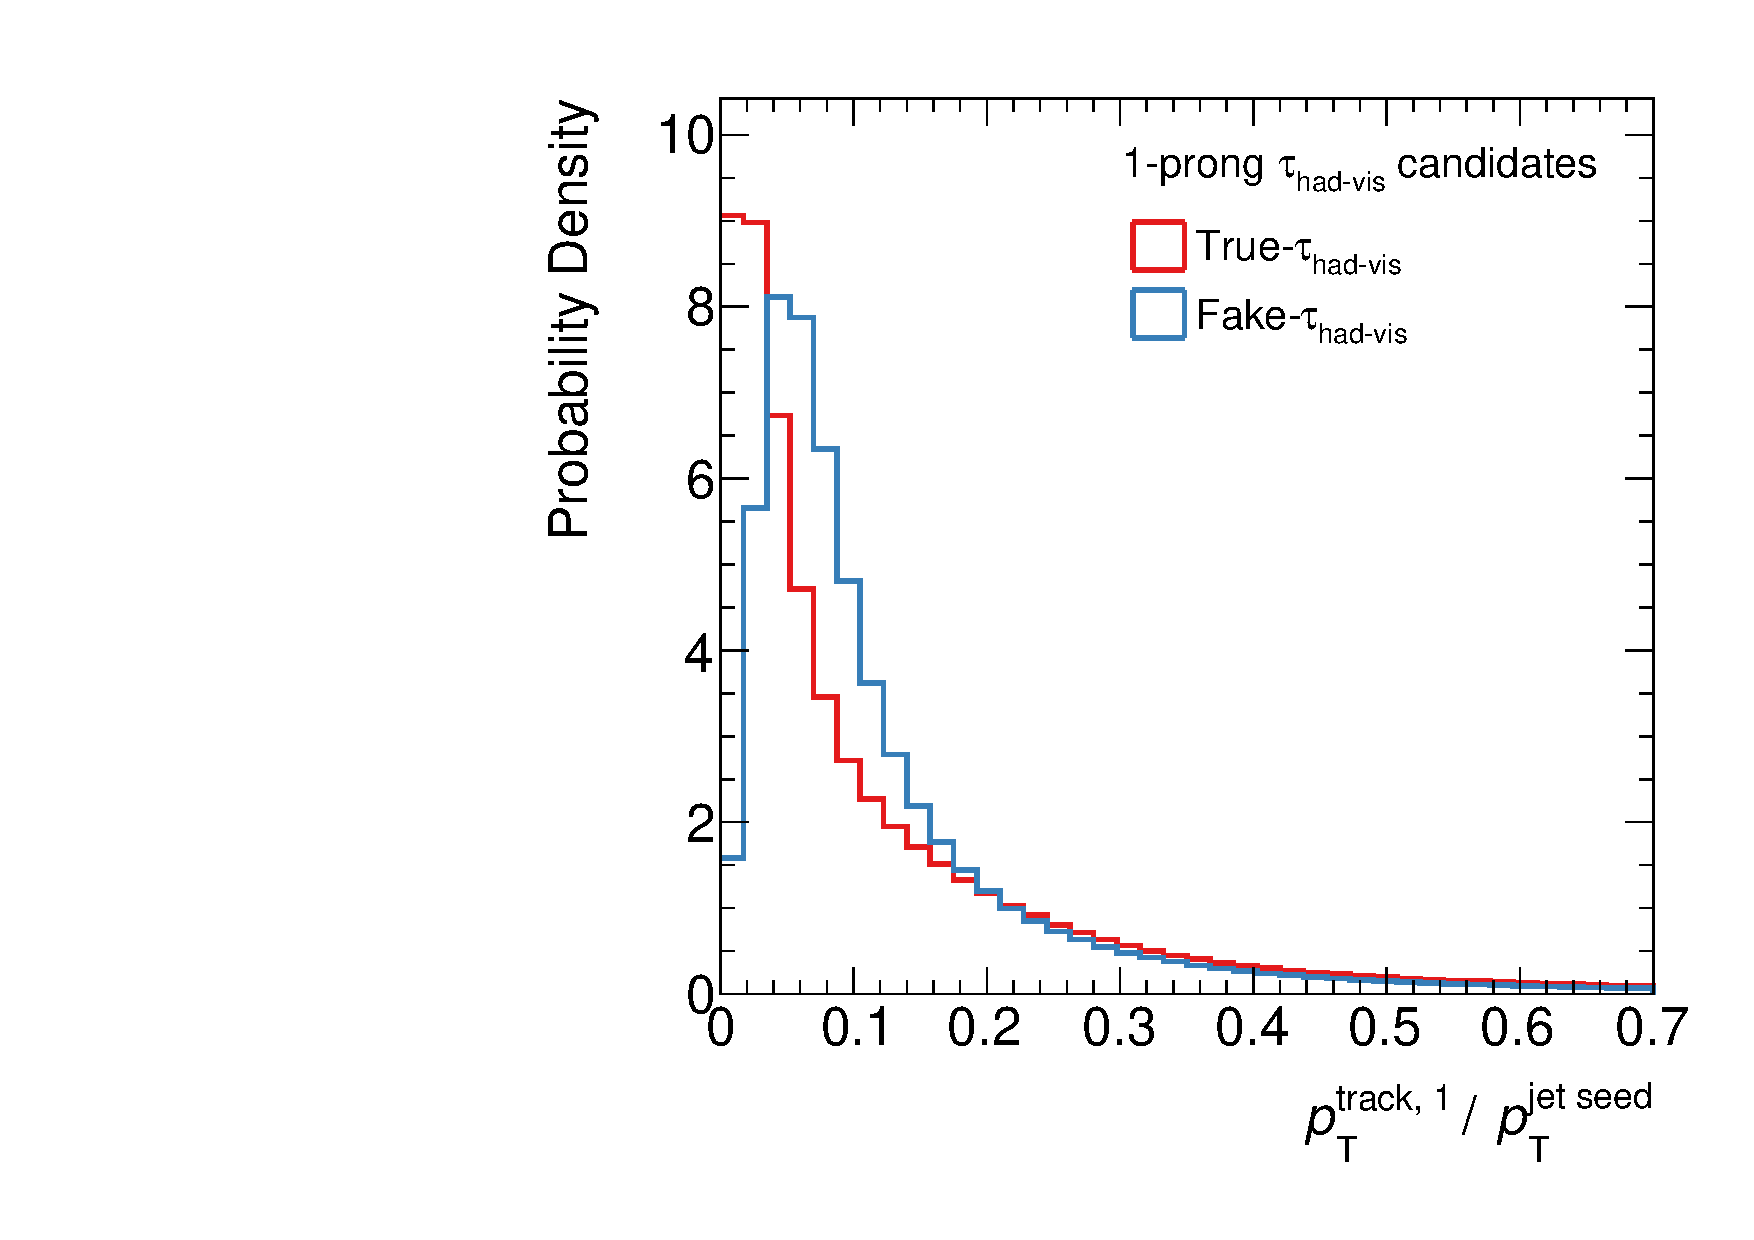
\includegraphics[width=\textwidth]{tauid/invars/invars_trk1relpt_1P}
    \subcaption{}%
    \label{fig:tauid_low_level_variables_track1}
  \end{subfigure}%
  \begin{subfigure}{0.33\textwidth}
    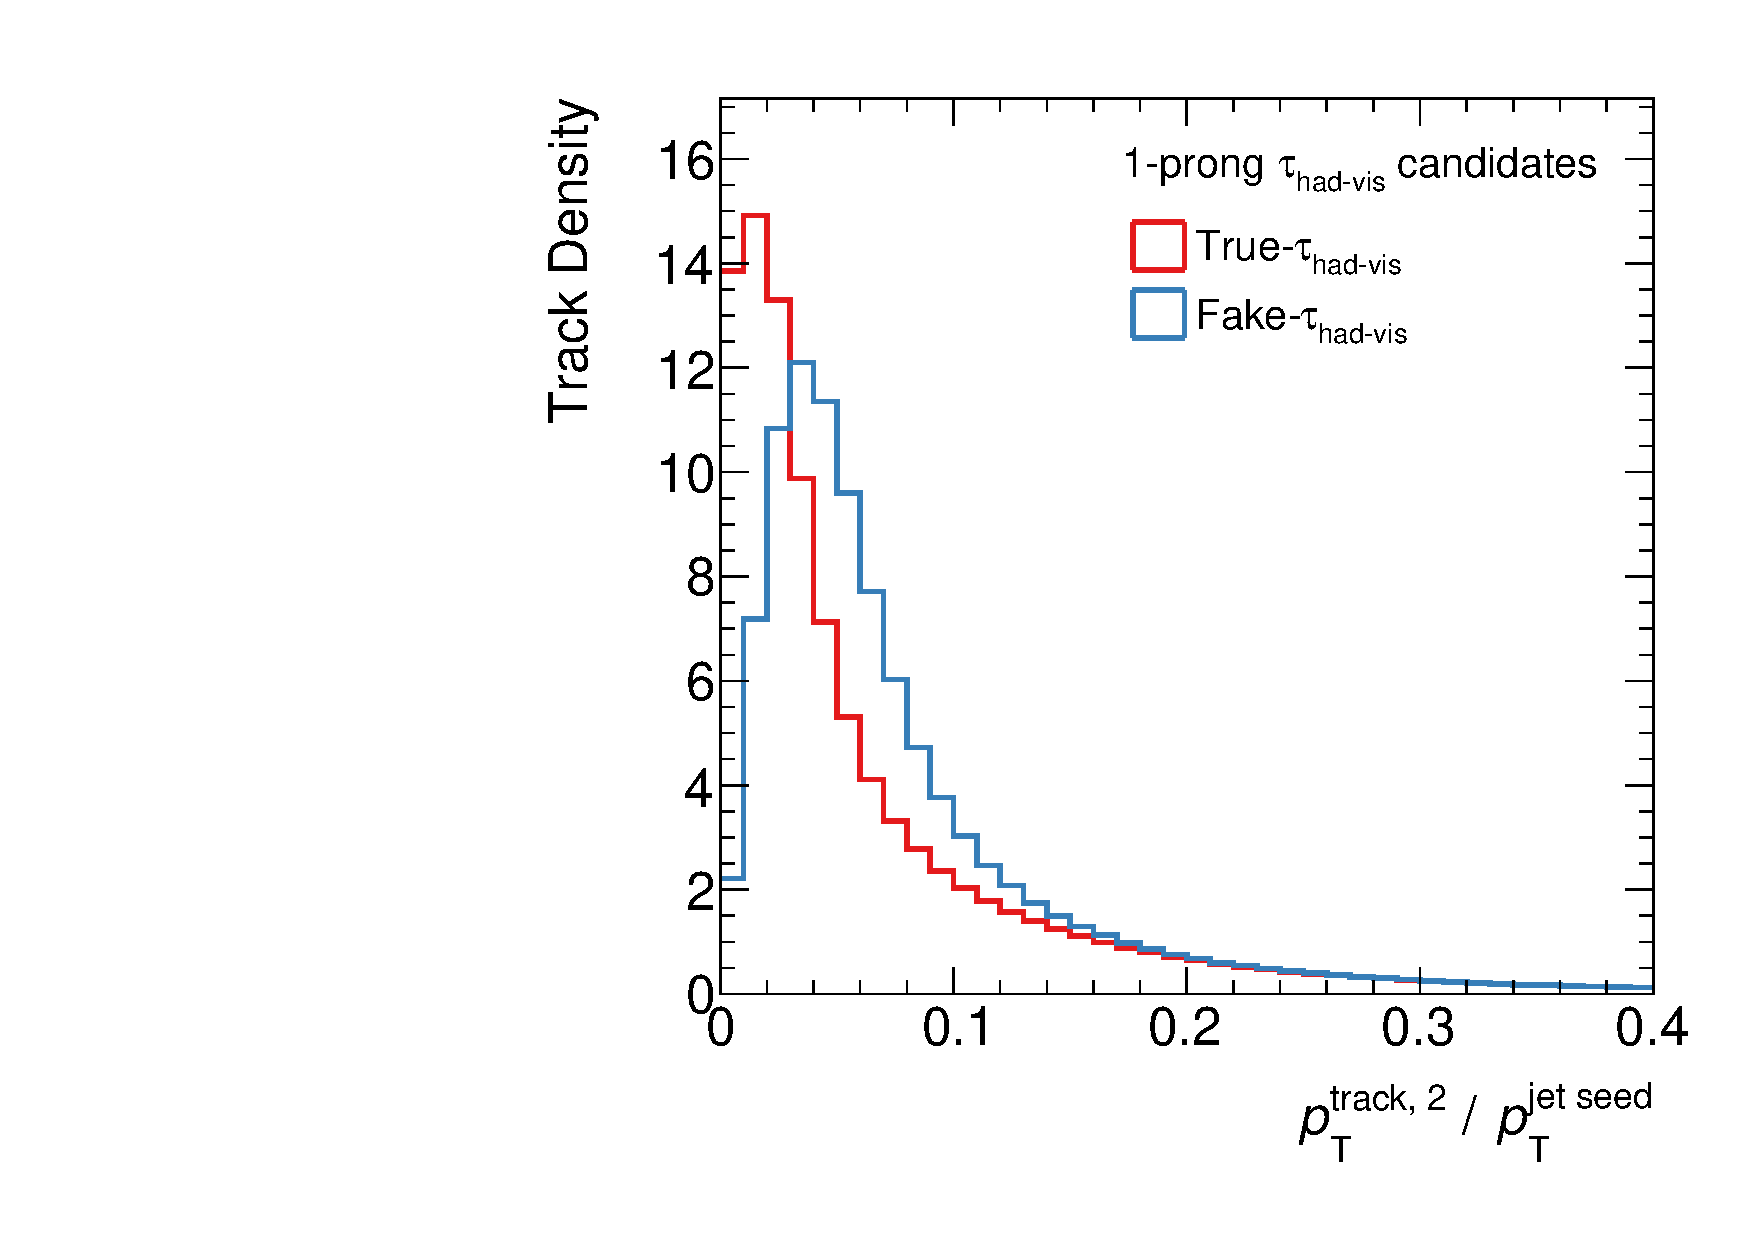
\includegraphics[width=\textwidth]{tauid/invars/invars_trk2relpt_1P}
    \subcaption{}%
    \label{fig:tauid_low_level_variables_track2}
  \end{subfigure}

  \caption[Distributions of the transverse momenta of the three highest-\pT
  tracks associated to 1-prong \tauhadvis candidates.]{Distributions of the
    transverse momenta of the three highest-\pT tracks associated to 1-prong
    \tauhadvis candidates. For illustration purposes, the track \pT are
    normalised to the \pT of the jet seeding the \tauhadvis candidate.}%
  \label{fig:tauid_low_level_variables_track}
\end{figure}

The discrimination power of the RNN \tauid saturates after including the ten
highest-\pT tracks; therefore, the sequence of tracks is truncated at this point
to reduce the computational resources required for training and evaluation of
the networks.


\subsubsection{Cluster Input Variables}

Topo-clusters in the calorimeters are considered as inputs to the RNN \tauid if
they are constituents of the jet seeding the \tauhadvis reconstruction. All
clusters are calibrated using the local hadronic calibration to account for the
non-compensating nature of the calorimeters, energy deposition in calorimeter
cells not part of the cluster, and energy loss in inactive
material~\cite{PERF-2014-07}.

The inclusion of the $E_{\text{T}}^{\text{cluster}}$,
$\Delta \eta^{\text{cluster}}$, $\Delta \phi^{\text{cluster}}$, and
$p_{\text{T}}^{\text{jet seed}}$ observables
(cf.~\Cref{tab:tauid_input_variables}) follow from considerations
similar to those for charged-particle tracks. In addition, information
on the position and shape of showers in the calorimeters is included
in the form of cluster moments~\cite{PERF-2014-07}, targeting the
differences between electromagnetic and hadronic showers. These
cluster moments include the longitudinal location of the cluster
barycentre, $\lambda_{\text{cluster}}$, and the lateral and
longitudinal extension of the cluster,
$\langle r^2 \rangle_{\text{cluster}}$ and
$\langle \lambda^2 \rangle_{\text{cluster}}$, respectively. For
illustration, the \ET of the three highest-\ET clusters is shown
in~\Cref{fig:tauid_low_level_variables_cluster} for 3-prong \tauhadvis
candidates.

\begin{figure}[htbp]
  \centering

  \begin{subfigure}{0.33\textwidth}
    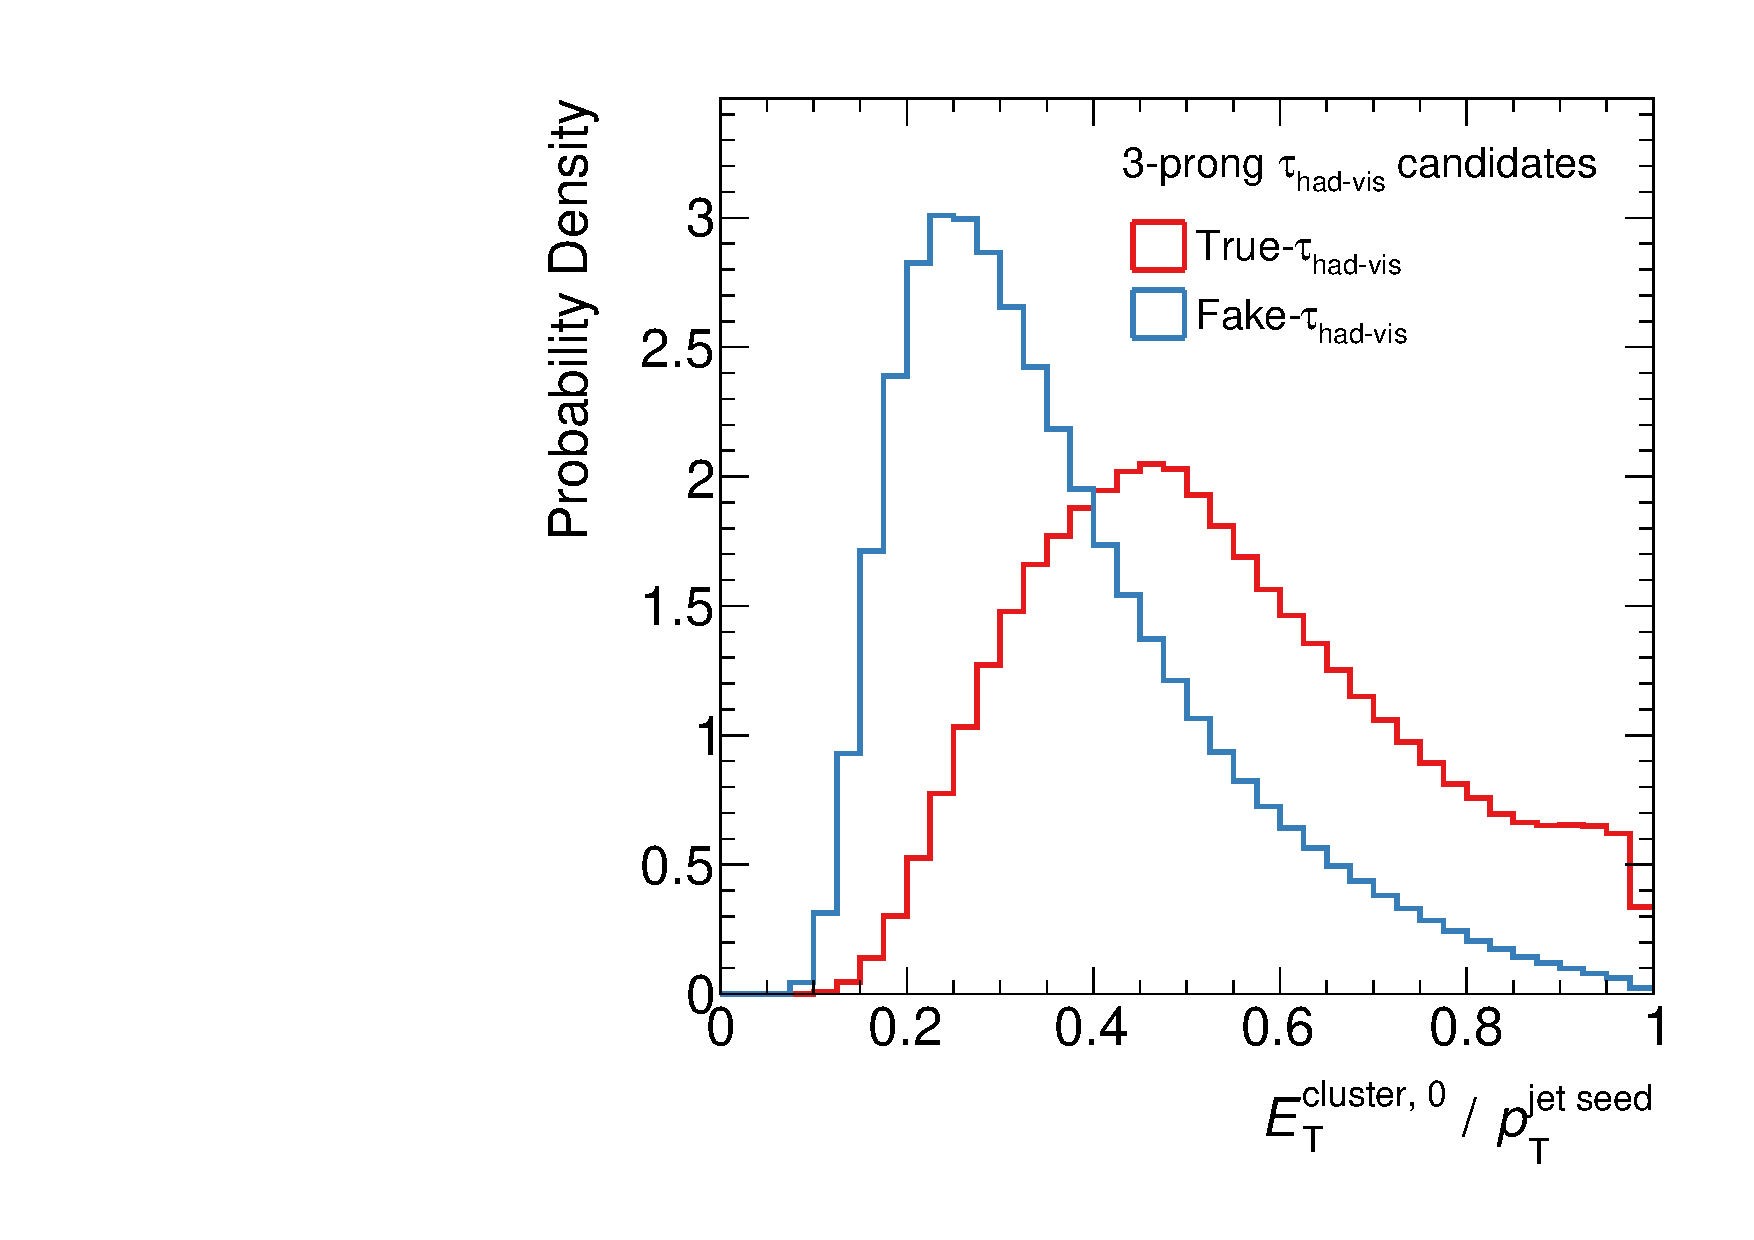
\includegraphics[width=\textwidth]{tauid/invars/invars_cls0relet_3P}
    \subcaption{}%
    \label{fig:tauid_low_level_variables_cluster0}
  \end{subfigure}%
  \begin{subfigure}{0.33\textwidth}
    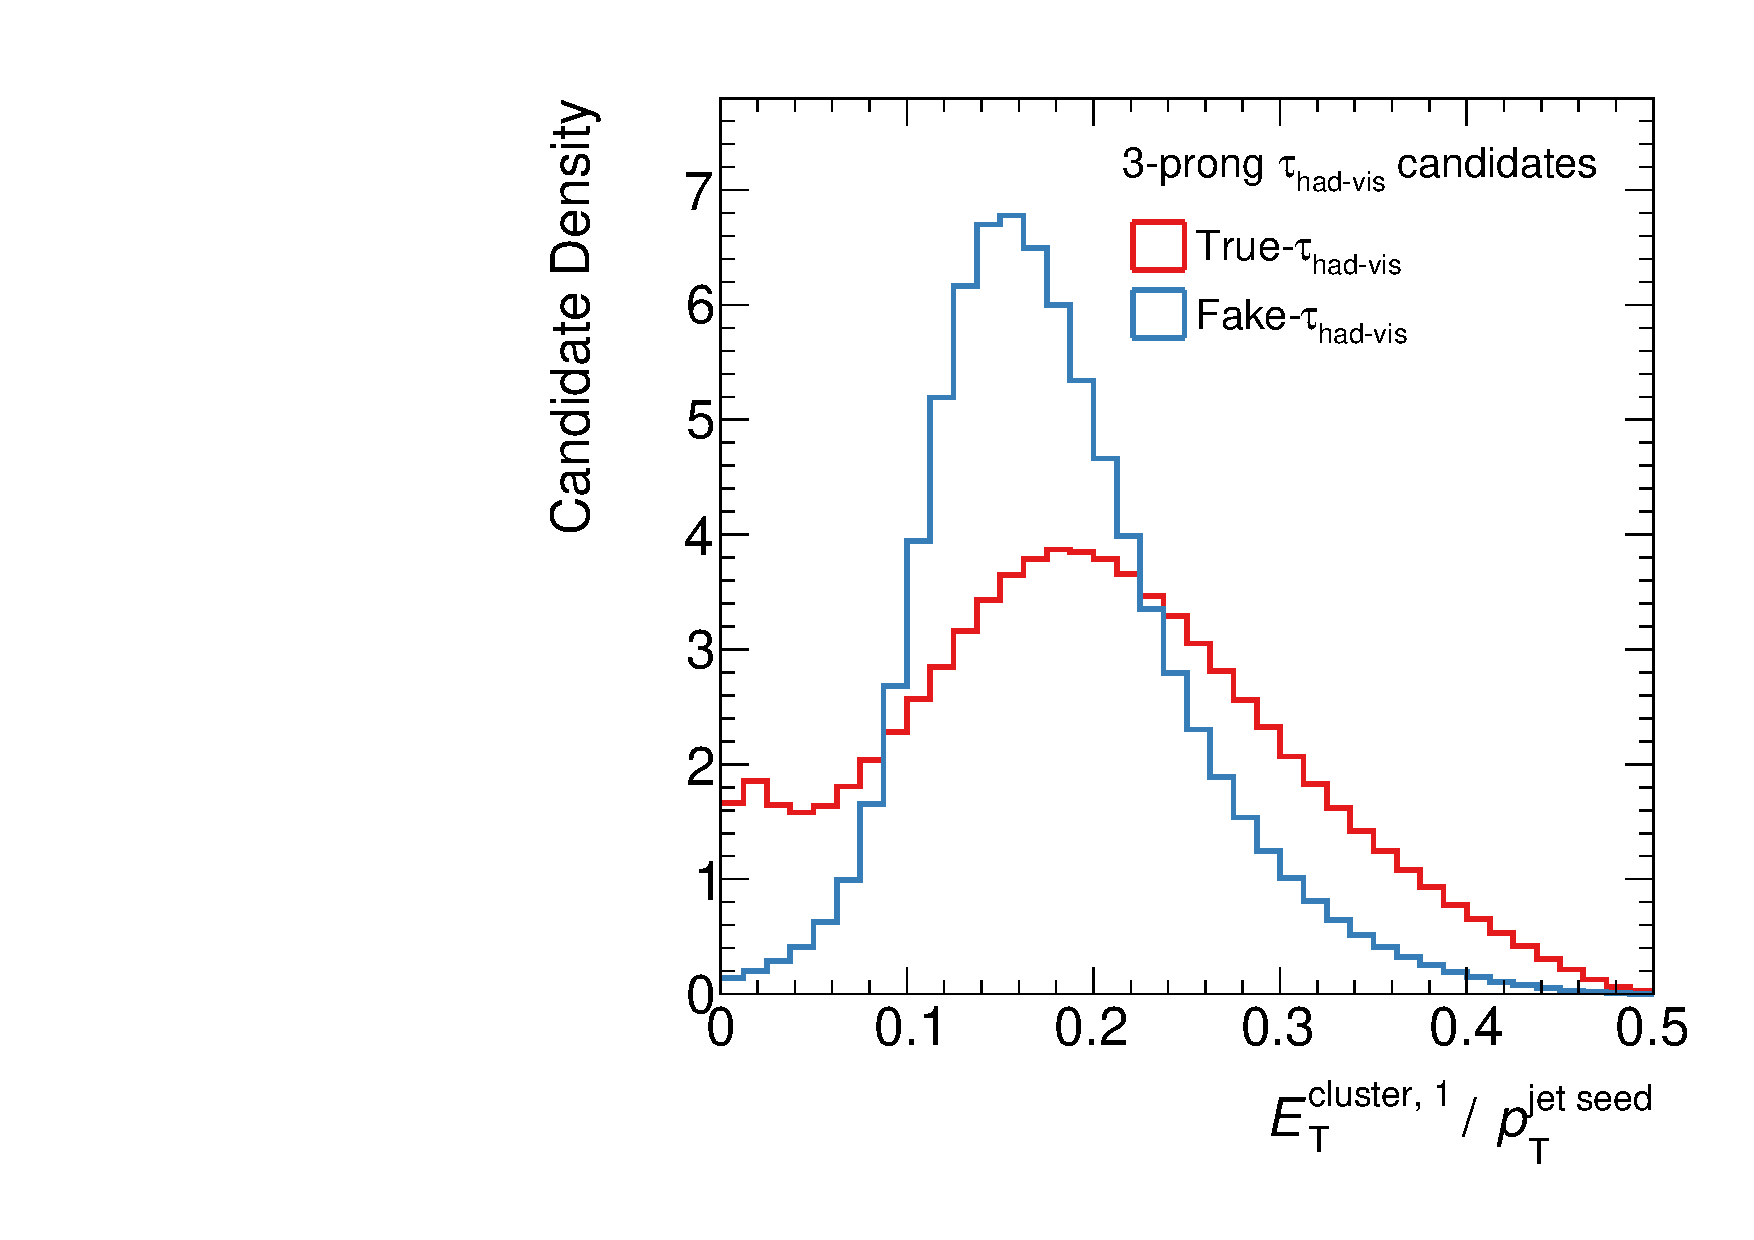
\includegraphics[width=\textwidth]{tauid/invars/invars_cls1relet_3P}
    \subcaption{}%
    \label{fig:tauid_low_level_variables_cluster1}
  \end{subfigure}%
  \begin{subfigure}{0.33\textwidth}
    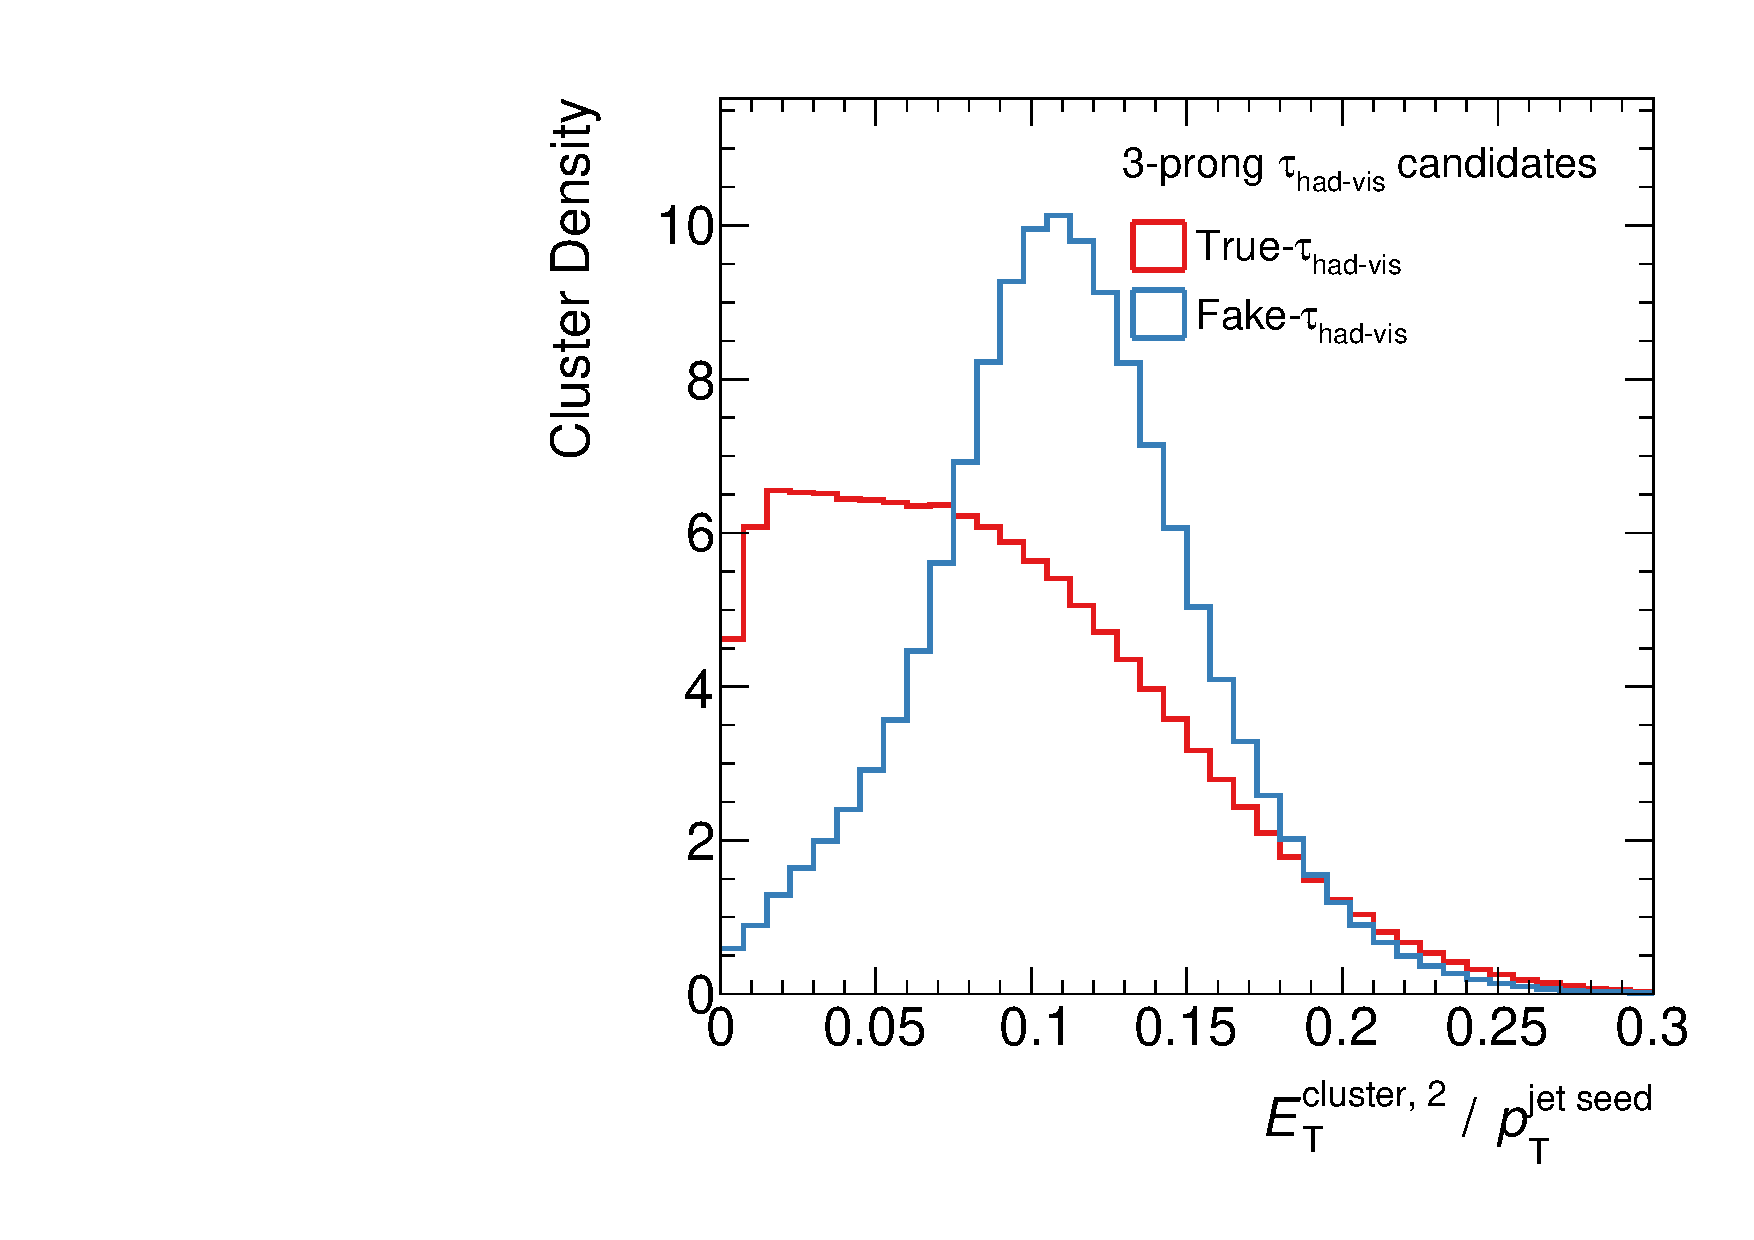
\includegraphics[width=\textwidth]{tauid/invars/invars_cls2relet_3P}
    \subcaption{}%
    \label{fig:tauid_low_level_variables_cluster2}
  \end{subfigure}

  \caption[Distributions of the transverse energy of the three highest-\ET
  clusters associated to 3-prong \tauhadvis candidates.]{Distributions of the
    transverse energies of the three highest-\ET clusters associated to 3-prong
    \tauhadvis candidates. For illustration purposes, the cluster \ET are
    normalised to the \pT of the jet seeding the \tauhadvis candidate.}%
  \label{fig:tauid_low_level_variables_cluster}
\end{figure}

The classification performance of the RNN \tauid saturates after the inclusion
of the six highest-\ET clusters, thus the sequence of input clusters is
truncated at this point.


\subsection{Network Architecture}

The network architecture adopted for the RNN \tauid is shown
schematically in~\Cref{fig:tauid_network_architecture}. The network
consists of three branches, each one dedicated to one type of
input. The high-level variables, track inputs, and cluster inputs are
first processed independently in their respective branches. These
branches are then merged and reduced to a single output node that is
used to define the \tauid working points. The network is implemented
using the \textsc{Keras} library~\cite{keras} with the
\textsc{TensorFlow}
backend~\cite{tensorflow2015-whitepaper}.\footnote{\textsc{Keras}
  v2.2.0 and \textsc{TensorFlow} v1.8.0 are used.} Layers use the
default configurations of \textsc{Keras} unless indicated otherwise. A
description of the network architecture is given in the following.

\begin{figure}[htbp]
  \centering

  \vspace*{0.2em}

  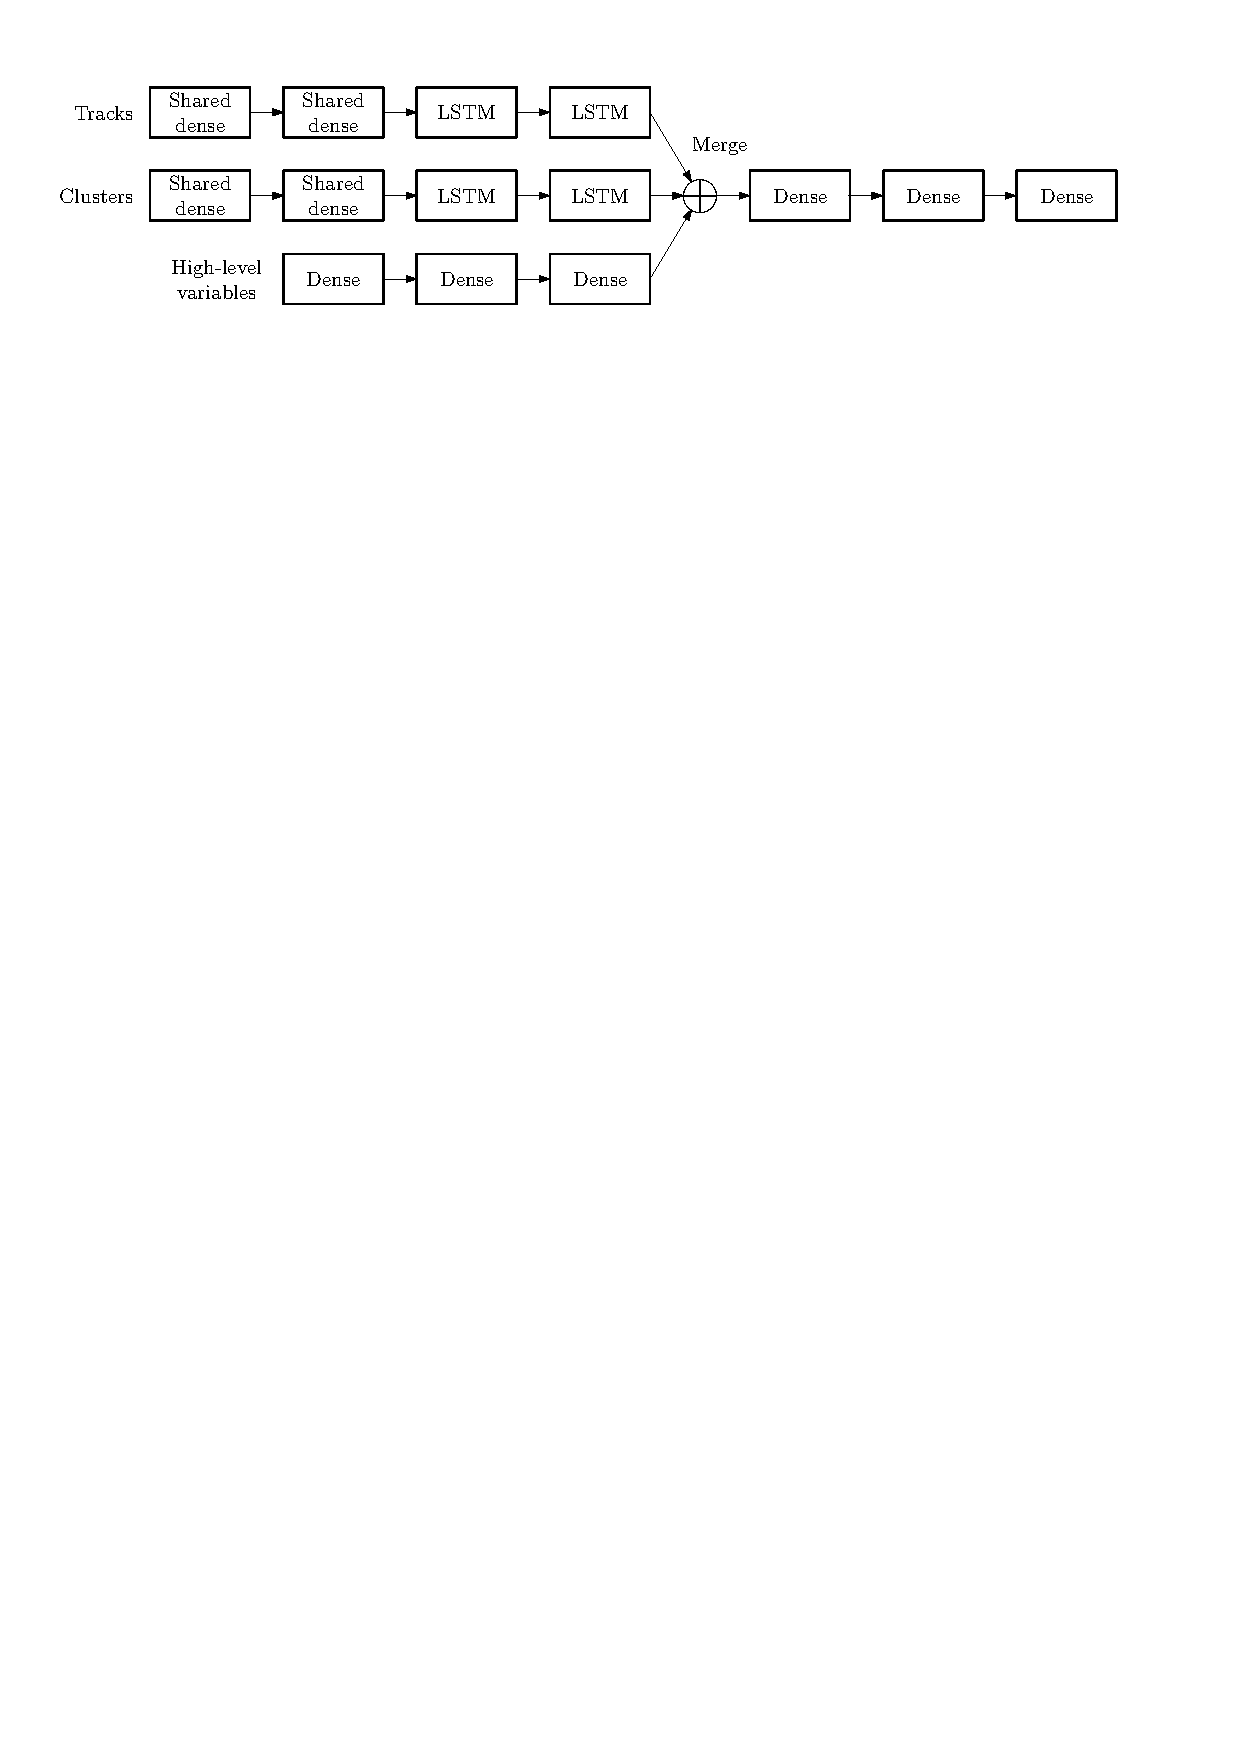
\includegraphics[width=0.98\textwidth]{tauid/pubnote/rnn_network_architecture}

  \vspace*{0.2em}

  \caption[Network architecture used for the RNN \tauid algorithm.]{Network
    architecture used for the RNN \tauid algorithm. Individual layers of the
    network are depicted as rectangles. The figure is adapted from
    Ref.~\cite{ATL-PHYS-PUB-2019-033}.}%
  \label{fig:tauid_network_architecture}
\end{figure}

The branch of the network operating on high-level input variables
consists of three fully-connected (\emph{dense}) layers with 128, 128,
and 16 units each. The \ReLU~\cite{nair:relu} activation function is
used in all layers.

The branches operating on track and cluster inputs are structured
identically. Tracks (clusters) are provided to the network as sequences of
vectors, each vector consisting of the values of the input variables for a given
track (cluster). The track and cluster sequences are given in descending
$p_{\text{T}}^{\text{track}}$ and $E_{T}^{\text{cluster}}$ order,
respectively. First, the sequences are passed through two fully-connected layers
with shared weights (\emph{shared dense}).  These layers have 32 units each and
use the \ReLU activation function. \emph{Shared dense} layers map input
sequences, $(\myvec{x}_t)_{t=1}^{N}$, to output sequences of the same length,
$(\myvec{y}_t)_{t=1}^{N}$, using transformations of the form
\begin{align*}
  \myvec{y}_t = \myvec{\phi}(\myvec{W} \myvec{x}_t + \myvec{b}) \,\text{,}
\end{align*}
where $\myvec{W}$ and $\myvec{b}$ are trainable weight matrices and bias
vectors, respectively, and $\myvec{\phi}$ is the activation function.  Notably,
the weights and biases do not depend on the index~$t$, meaning the weights and
biases are the same (i.e.\ shared) for all elements of the sequence. The
\emph{shared dense} layers produce intermediate representations of the track and
cluster sequences for further computation.

The transformed sequences of tracks and clusters pass through two recurrent
layers based on an LSTM architecture (cf.\ \Cref{sec:rnn}). The first LSTM layer
maps the input sequence to an output sequence of the same length. In contrast to
\emph{shared dense} layers, LSTM layers have an internal state that is updated
as elements of the sequence are processed. Therefore, information about elements
occurring in the sequence can be exploited when processing subsequent
elements. The second LSTM layer repeats the process, however, all except the
last element of the output sequence are discarded, thereby encoding the input
sequence into an output of fixed size. The size of the internal state and
outputs of the LSTM layers are chosen to be the same and correspond to 32 units
for the first and 24 units for the second LSTM layer.

Finally, the outputs of the three branches are concatenated
(\emph{Merge}) and passed through three fully-connected layers with
sizes of 64, 32, and 1 units. The \ReLU (sigmoid) activation function
is used for the hidden layers (output layer). The entire model
consists of approximately \num{56000} trainable parameters.


\subsection{Network Training and Evaluation}

Two separate networks are trained for the classification of 1- and
3-prong \tauhadvis candidates. The samples of \tauhadvis candidates
are partitioned into a training (\SI{40}{\percent}), validation
(\SI{10}{\percent}), and testing datasets (\SI{50}{\percent}). The
trainable parameters of the networks are determined by minimising the
binary cross-entropy loss on the training dataset. The loss of the
network is monitored on the validation datasets and is used to steer
the training procedure.

SGD with momentum is used for loss minimisation. Prior to the training,
transformations are applied to input variables for better conditioning of the
minimisation problem. The learning rate of the optimiser is reduced when the
validation loss did not improve for four successive training epochs, where an
epoch refers to a single pass over the training data. Similarly, the training is
stopped after ten epochs without improvements of the validation loss in which
case the model parameters resulting in the best validation loss are restored.

The trained NNs are implemented for evaluation during offline
event reconstruction in the \textsc{Athena} software
suite~\cite{ATL-SOFT-PUB-2021-001} using the \textsc{lwtnn}
library~\cite{lwtnn}.

The classification score computed by the RNN \tauid is transformed to
be approximately uniformly distributed for \truetauhadvis
candidates. The transformed score, referred to as the RNN score and
shown in~\Cref{fig:flattened_rnnscore}, allows the definition of working
points for a specific \truetauhadvisC identification efficiency target by
applying a threshold to the score. Moreover, the transformation is
derived in bins of \tauhadvis \pT (calorimeter-based \pT estimate at
LC scale) and the average number of interactions per bunch crossing,
$\mu$, to ensure that the \truetauhadvisC efficiencies of working
points remains approximately constant with changing \tauhadvis \pT or
pile-up conditions. The same procedure is applied for the BDT-based
\tauid algorithm.

\begin{figure}[htbp]
  \centering

  \begin{subfigure}{0.498\textwidth}
    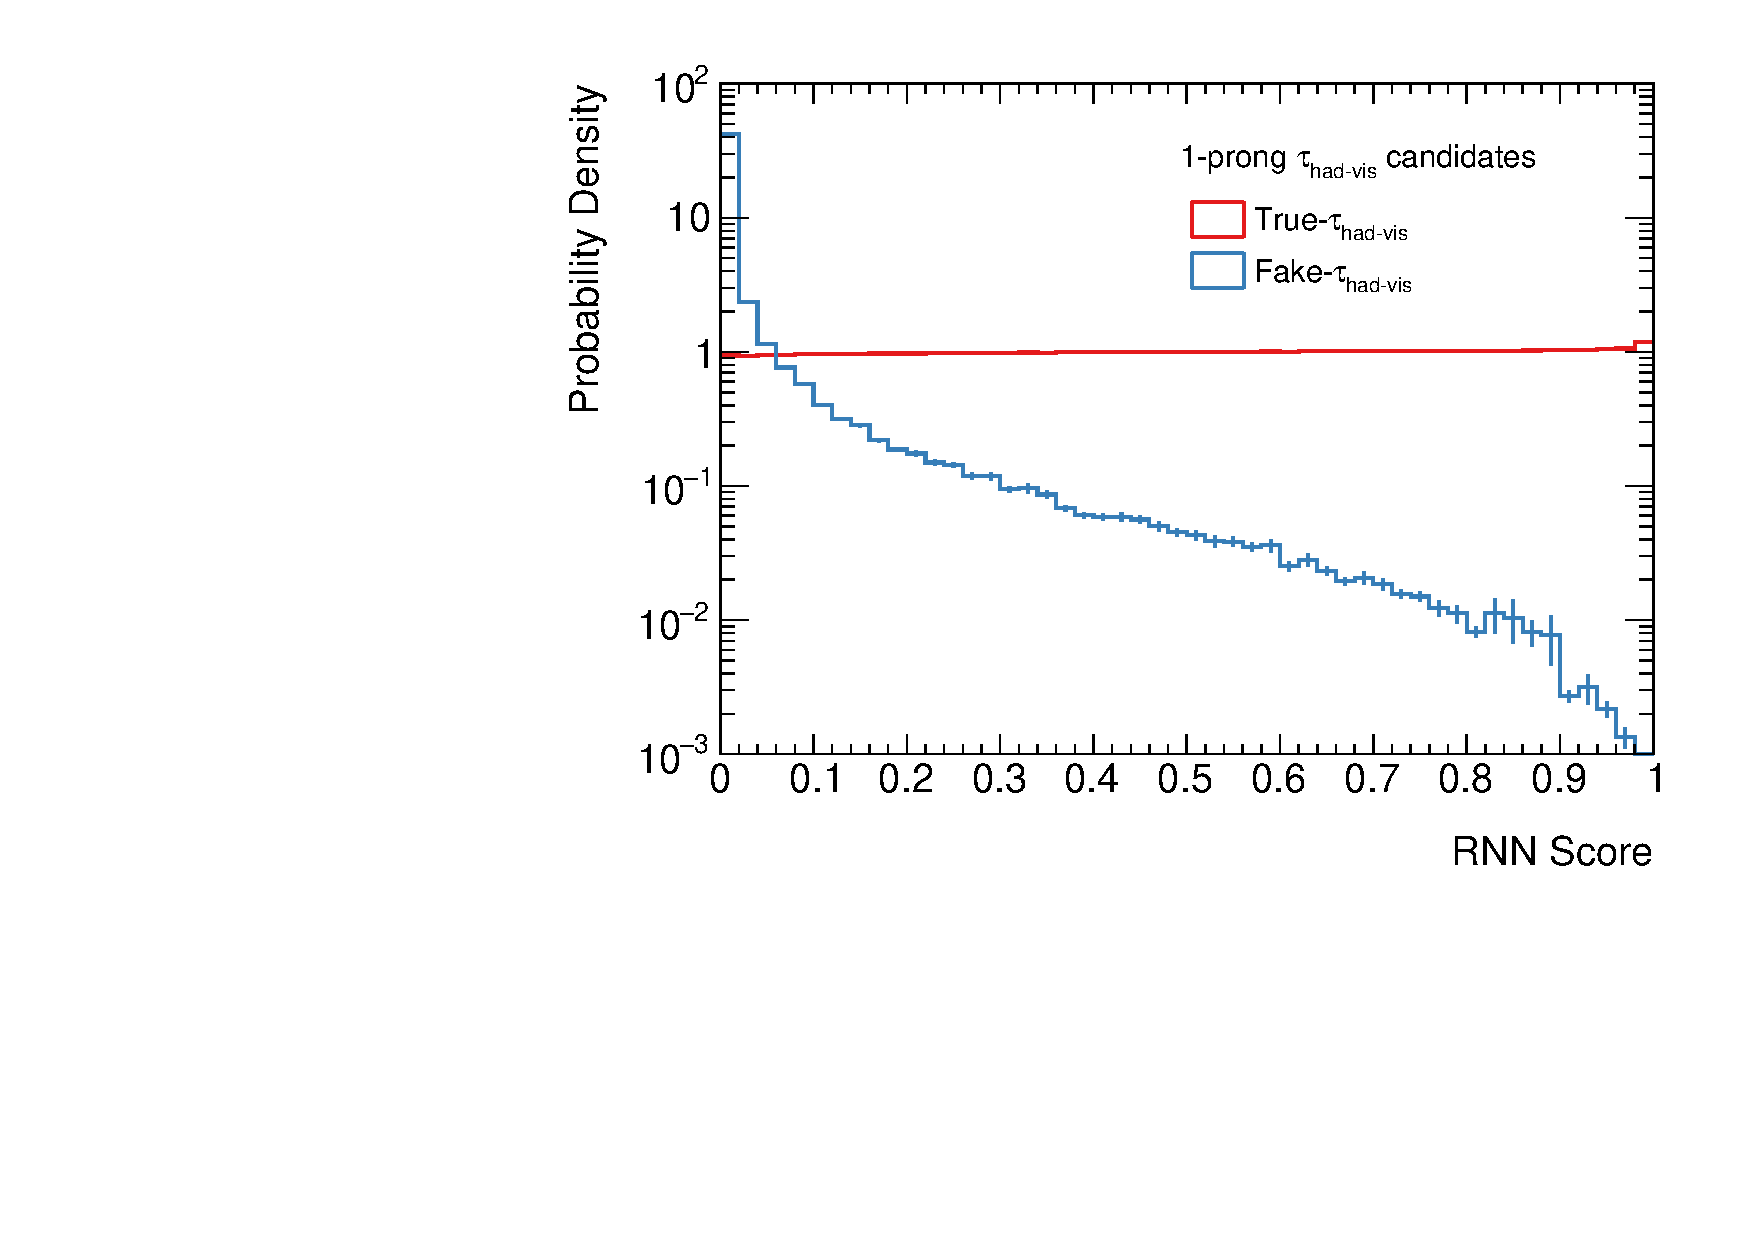
\includegraphics[width=\textwidth]{tauid/rnnscore_1p}
    \subcaption{}
  \end{subfigure}\hfill%
  \begin{subfigure}{0.498\textwidth}
    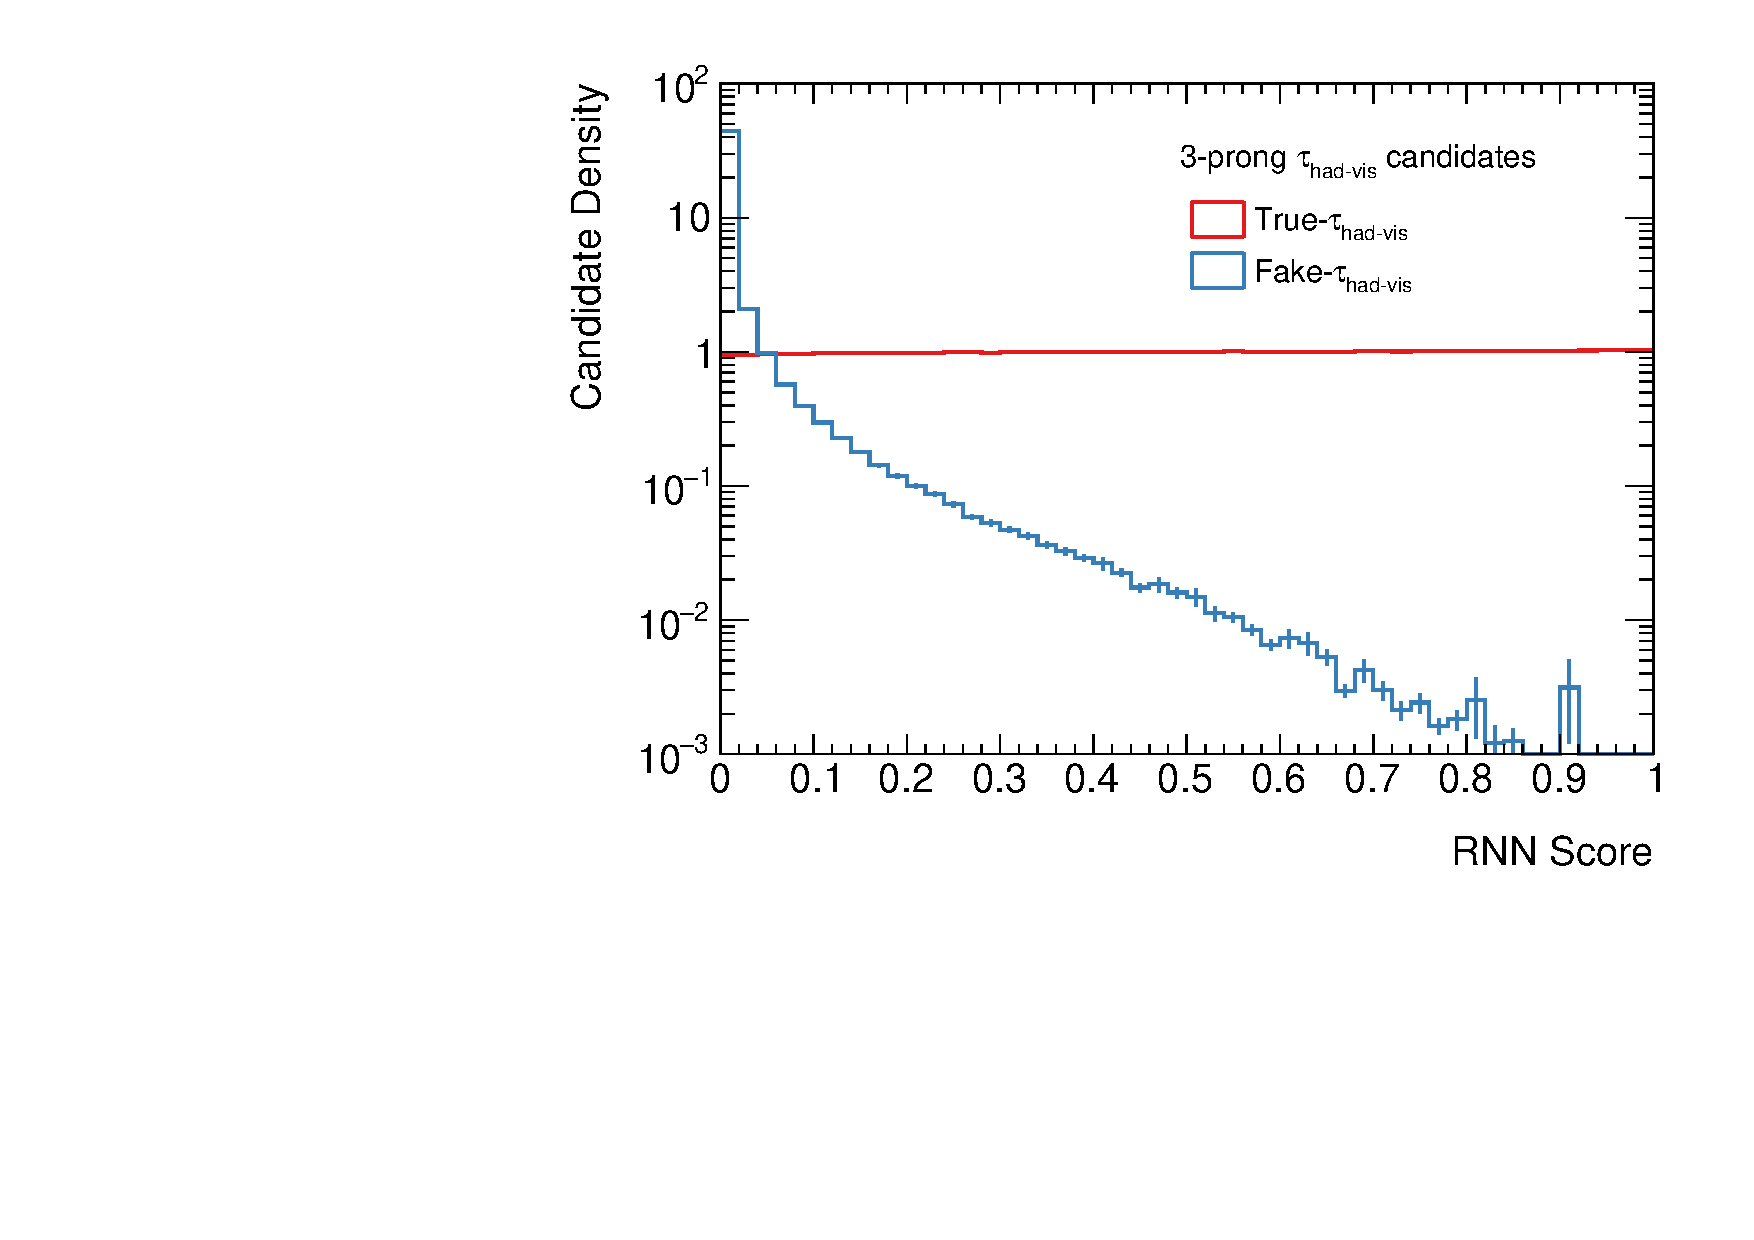
\includegraphics[width=\textwidth]{tauid/rnnscore_3p}
    \subcaption{}
  \end{subfigure}

  \caption[Distributions of the RNN score for 1-prong and 3-prong \tauhadvis
  candidates.]{Distributions of the RNN score for 1-prong (a) and 3-prong (b)
    \tauhadvis candidates. The RNN scores are shown after transformations that
    ensure that the scores of \truetauhadvis are approximately uniformly
    distributed. The figures are adapted from
    Ref.~\cite{ATL-PHYS-PUB-2019-033}.}%
  \label{fig:flattened_rnnscore}
\end{figure}

%%% Local Variables:
%%% mode: latex
%%% TeX-master: "../../phd_thesis"
%%% End:
